\documentclass[10pt,a4paper]{article}

\usepackage[english]{babel}
\usepackage[utf8]{inputenc}
\usepackage[T1]{fontenc}
\usepackage[a4paper, margin=2cm]{geometry}
\usepackage{amsmath,amsfonts,amssymb}
\usepackage[colorlinks]{hyperref}
\usepackage{multicol}
\usepackage{graphicx}
\usepackage{float}
\usepackage{booktabs}
\usepackage{lipsum}

\usepackage[round]{natbib}
\bibliographystyle{abbrvnat}

\usepackage{fancyhdr}
\pagestyle{fancy}
\fancyhead[L]{02460-2026 Mini-project 1}
\fancyhead[R]{s039894, s271828 \& s314159}

% For including code
% From https://www.overleaf.com/learn/latex/Code_listing
\usepackage{listings}
\usepackage{xcolor}

\definecolor{codegreen}{rgb}{0,0.6,0}
\definecolor{codegray}{rgb}{0.5,0.5,0.5}
\definecolor{codepurple}{rgb}{0.58,0,0.82}
\definecolor{backcolour}{rgb}{0.95,0.95,0.92}

\lstdefinestyle{mystyle}{
    backgroundcolor=\color{backcolour},
    commentstyle=\color{codegreen},
    keywordstyle=\color{magenta},
    numberstyle=\tiny\color{codegray},
    stringstyle=\color{codepurple},
    basicstyle=\ttfamily\footnotesize,
    breakatwhitespace=false,
    breaklines=true,
    captionpos=b,
    keepspaces=true,
    numbers=left,
    numbersep=5pt,
    showspaces=false,
    showstringspaces=false,
    showtabs=false,
    tabsize=2,
    upquote=true
}

\lstset{language=Python, style=mystyle}

\begin{document}

%%% Main text part %%%

\section*{Mini-project 1 in Advanced Machine Learning (02460)}
by Marcus Christoffersen (s224750), Bob (s271828) \& Eve (s314159) on 05 March 2026

\begin{multicols}{2}

    % -------------------------------------------------------------------
    \subsection*{Part A: VAE Priors}
    % -------------------------------------------------------------------

    We train VAEs on binarised MNIST with three priors: standard Gaussian,
    a 10-component MoG, and a flow-based prior (8 affine coupling layers).
    For non-Gaussian priors the KL is estimated via Monte Carlo.
    Figure~\ref{fig:prior_posterior} shows t-SNE projections of prior and
    aggregate posterior samples. The Gaussian prior forms a unimodal blob
    misaligned with the multi-modal posterior; MoG and Flow priors
    learn to better align with the digit-class structure.
    Test ELBOs (mean$\pm$std, 5 runs): Gaussian $-88.77\pm0.69$,
    MoG $-88.16\pm0.67$, Flow $-88.05\pm0.38$.
    Differences are small, likely because the decoder capacity is
    the binding constraint: once the reconstruction term is saturated,
    prior flexibility yields diminishing returns.
    The flow prior also shows lower variance, suggesting a more stable training objective.

    \begin{figure}[H]
        \centering
        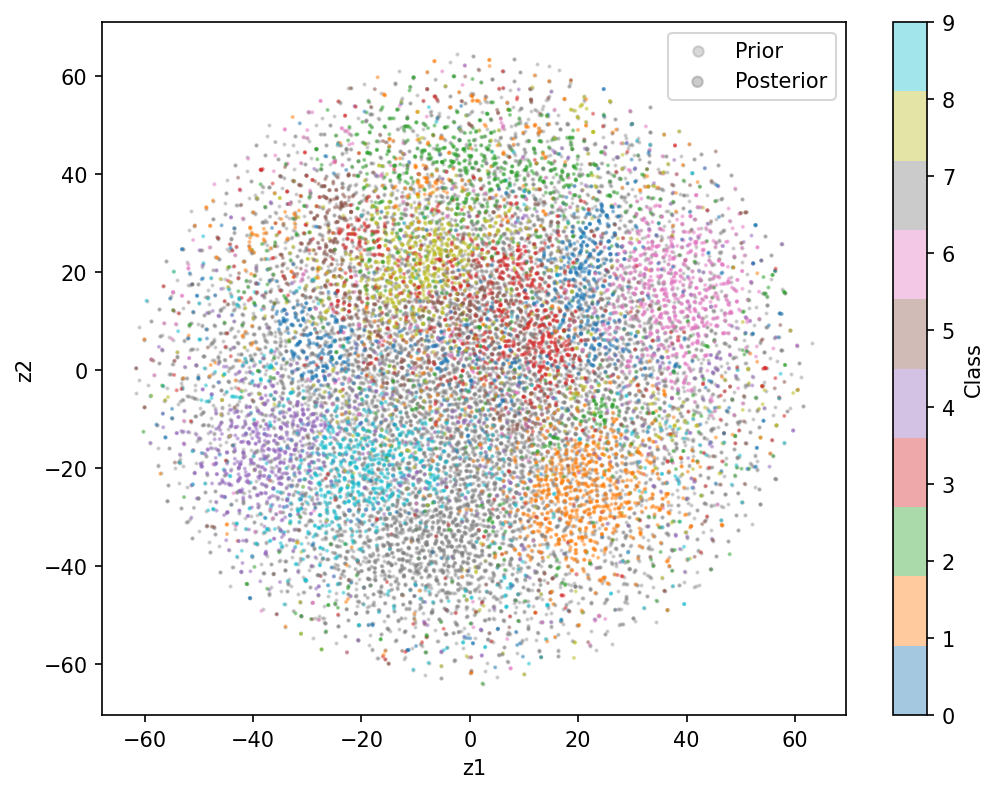
\includegraphics[width=0.32\columnwidth]{Figures/vae/gauss_prior_posterior}
        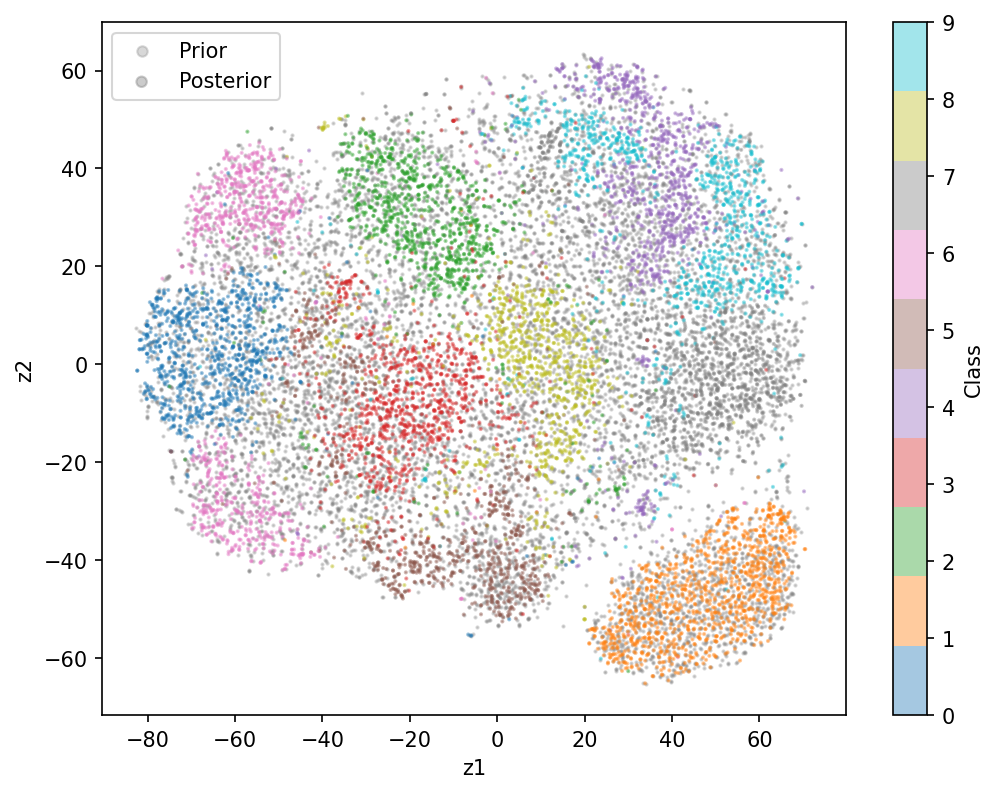
\includegraphics[width=0.32\columnwidth]{Figures/vae/mog_prior_posterior}
        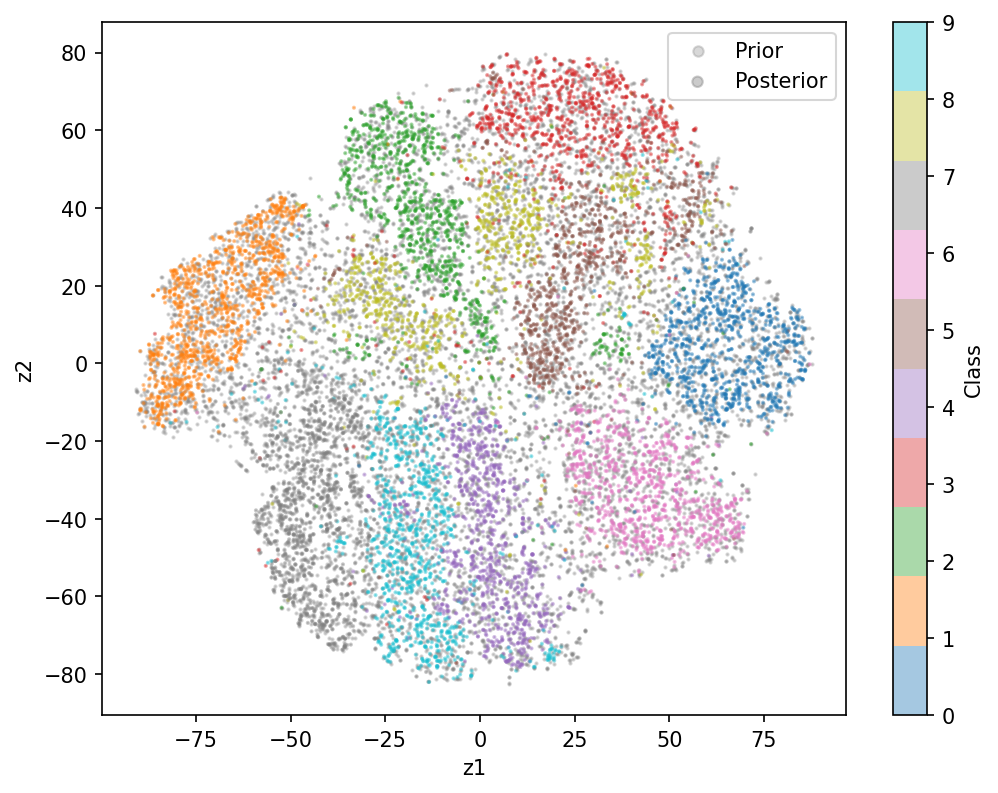
\includegraphics[width=0.32\columnwidth]{Figures/vae/flow_prior_posterior}
        \caption{Prior vs.\ aggregate posterior for Gaussian (left), MoG (mid), Flow (right).}
        \label{fig:prior_posterior}
    \end{figure}

    % -------------------------------------------------------------------
    \subsection*{Part B: Sampling Quality}
    % -------------------------------------------------------------------

    % TODO: Architecture description + discussion text
    \lipsum[4]

    \begin{figure}[H]
        \centering
        
\includegraphics[width=0.28\columnwidth]{Figures/vae/mog_samples_4}
        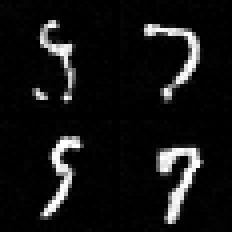
\includegraphics[width=0.28\columnwidth]{Figures/ddpm/ddpm_samples_4}
        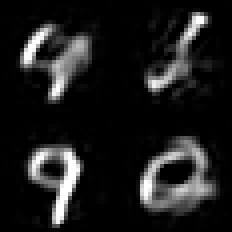
\includegraphics[width=0.28\columnwidth]{Figures/ddpm/latent_ddpm_samples_b1e-3_4}
        \caption{$2{\times}2$ samples: VAE MoG (left), DDPM U-Net (mid), Latent DDPM $\beta\!=\!10^{-3}$ (right).}
        \label{fig:samples}
    \end{figure}

    \begin{table}[H]
        \caption{FID ($\downarrow$) and sampling speed on standard MNIST ($N\!=\!1000$).}
        \begin{center}
            \begin{tabular}{lcc}
                \toprule
                Model & FID & Samp./s \\
                \midrule
                VAE (Gaussian)                  & 42.30  & 13{,}179 \\
                DDPM (U-Net)                    & 36.96  & 35       \\
                Lat.\ DDPM $\beta\!=\!10^{-6}$  & 115.15 & 8{,}405  \\
                Lat.\ DDPM $\beta\!=\!10^{-3}$  & 81.91  & 8{,}613  \\
                Lat.\ DDPM $\beta\!=\!0.1$      & 88.80  & 8{,}584  \\
                Lat.\ DDPM $\beta\!=\!1$        & 153.18 & 8{,}861  \\
                \bottomrule
            \end{tabular}
        \end{center}
    \end{table}

    \begin{figure}[H]
        \centering
        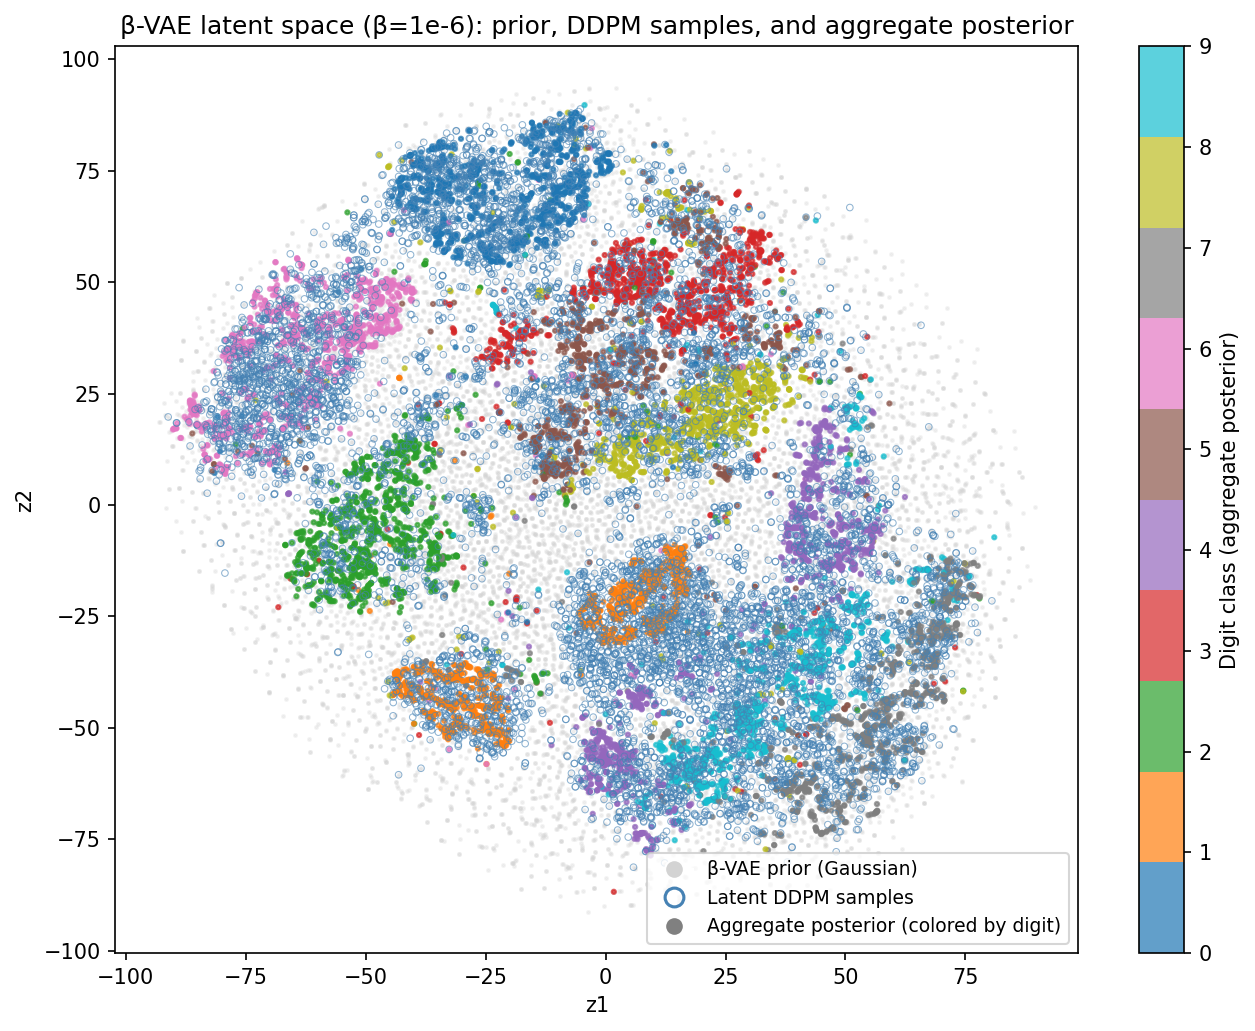
\includegraphics[width=0.65\columnwidth]{Figures/ddpm/latent_ddpm_prior_posterior}
        \caption{Latent space ($\beta\!=\!10^{-6}$): Gaussian prior (grey), DDPM latents (blue), aggregate posterior (coloured).}
        \label{fig:latent_space}
    \end{figure}

    % TODO: Latent space discussion
    \lipsum[5-6]

\end{multicols}

\newpage

%%% Code snippet part %%%

\section*{Code snippets}

% TODO: (1) VAE ELBO with non-Gaussian prior (MoG MC KL fallback)

% TODO: (2) Central parts of Flow implementation

% TODO: (3) DDPM ELBO implementation

% TODO: (4) DDPM sampling algorithm

% TODO: (5) Latent DDPM training and sampling steps

\newpage

%%% AI declaration %%%

\section*{Declaration of use of generative AI}

This declaration \textbf{must} be filled out and included as the 3rd page of the document. The questions apply to all parts of the work, including research, project writing, and coding.
\begin{itemize}
\item I/we have used generative AI tools: [yes / no]
\end{itemize}
If you answered \emph{yes}, please complete the following sections. List the generative AI tools you have used:
\begin{itemize}
\item
\end{itemize}
Describe how the tools were used:
\begin{description}
\item[What did you use the tool(s) for?]
\item[At what stage(s) of the process did you use the tool(s)?]
\item[How did you use or incorporate the generated output?]
\end{description}

\newpage

%%% Bibliography %%%

\bibliography{template}

\end{document}
